Tout d'abord, il faut définir $P_{dBm}$. Le schéma du microphone qui nous est donné permet de réaliser les calculs.
%
ici photo
%

En effet, nous avons la relation suivante :
\begin{equation}
P_{dBm} = 10 \times \log(V_a^2 \times 1000) \ \text{avec}\ V_a = S \times P_a
\end{equation}
Cependant, la sensibilité que l'on nous donne est en dBv et pas en $V/P_a$, il faut donc la convertir. Nous savons que :\begin{equation}
    S = 20\times \log(\frac{S_{v/Pa}}{S_{ref}}) \ \text{avec}\  S_{ref} = 1 V/P_a
\end{equation} donc :
\begin{equation}
   S_{V/P_a} = S_{ref}*10^\frac{S}{20} 
\end{equation}
\begin{equation}
    \text{donc}\ V_m = S_{\frac{V}{P_a}} \times P_a
\end{equation} 
Pour $P_a$, nous utilisons la formule de $P_{SPL}$: 
\begin{equation}
    P_{SPL} = 20\times \log(\frac{P_a}{P_{ref}}) 
\end{equation}
d'où:
\begin{equation}
P_a = P_{ref} * 10^{\frac{P_{SPL}}{20}}
\end{equation}
Il ne reste que le gain à traiter, celui-ci s'exprime en dB dans les paramètres donnés, or, nous voulons l'exprimer sans unité ; nous obtenons alors 
\begin{equation}
    G_{SU} = 10^\frac{G}{20} \ \text{où} \ G_{SU} \ \text{est sans unité}
\end{equation}
Cela nous permet de trouver la formule finale : 
\textcolor{red}{
\begin{equation}
    P_{dBm} = 10 \times \log((G_{SU} \times S_{VPA} \times P_a)^2 \times 1000)
\end{equation}
}
En substituant avec les résultats précédents, on obtient :
\textcolor{red}{
\begin{equation}
    P_{dBm} = 20 \times \log(10^\frac{G}{20} \times S_{REF} \times 10^{\frac{S}{20}} \times P_{REF} \times 10^{\frac{P_{SPL}}{20}})+30
\end{equation}
}
Enfin, avec : \begin{itemize}
    \item $S_REF = 1$
    \item $P_REF = 20 \mu Pa$
    \item $G = 40 dB$
    \item $S = -48 dBV$
    \item $P_SPL = 80 dB SPL$
\end{itemize} 
On obtient : \textcolor{red}{$P_{dBm} = 8 dBm$}.
\newline\newline
À présent, nous avons la valeur de $P_{dBm}$ qui va nous servir de référence. Pour chaque signal, nous allons le décomposer en plusieurs « sous-signaux » à chaque fois que la valeur de référence est franchie. 
\newline
Par exemple, sur la figure \ref{Fig.1.2}, on distingue trois « sous-signaux » ou plages de signal différentes car la valeur de référence est franchie deux fois. Ensuite, chaque plage est traitée comme un nouveau signal et, si cette plage se trouve au-dessus de la valeur référence et dure plus d’une seconde, alors le son de cette plage est catalogué dans la catégorie bruit pénible. Sur cet exemple il y a donc deux sons acceptables (plages 1,3) et un son pénible (plage 2).
\newline
Enfin, pour chaque signal, on règle la taille des fenêtres d’analyse pour obtenir un résultat correct, contenant 2k+1 échantillons.
\begin{figure}[htb]
    \centering
    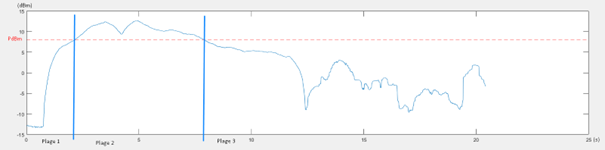
\includegraphics[width=0.8\textwidth]{Exemple_seuil_se_pénibilité.png}
    \caption{Exemple signal avec plages acceptables et pénibles}
    \label{Fig.1.2}
\end{figure}
